
%% Big Data Literary Review
%% 2015/08/26
%% by Will Hogan

\documentclass[10pt,journal,compsoc]{IEEEtran}

% *** CITATION PACKAGES ***
%
\ifCLASSOPTIONcompsoc
  % IEEE Computer Society needs nocompress option
  % requires cite.sty v4.0 or later (November 2003)
  \usepackage[nocompress]{cite}
    \usepackage{romannum}
    \usepackage{tcolorbox}
    \usepackage{amsmath}
    \usepackage[noend]{algpseudocode}
    \usepackage[]{algorithm2e}
    \usepackage{tcolorbox}
    \usepackage{graphicx}
\else
  \usepackage{cite}
\fi

\hyphenation{op-tical net-works semi-conduc-tor}

\begin{document}

\title{Big Data}

\author{Will~Hogan 
	\\{4th Year Software Development}
	\\{Research Methodologies in Computing and I.T.}}


\IEEEtitleabstractindextext{%
\begin{abstract}
In modern day computing, the term Big Data is used to describe large amounts of data and human made devices are creating and storing this data on a massive scale globally. The purpose of this review is to explore the world of Big Data and look at it from the ground up in terms of what data actually is, how it's structured and how it's used by organisations. We'll take an in depth look at Big Data Analytics and how Data Mining can be extremely useful for uncovering information relating to current trends or customer spending. We'll see why an important part of why organisations store and access Big Data is to yield benefits of which Cost Reduction and improved decision making would be considered key. Finally, we'll take a look at what direction Big Data will take in the immediate future and see how new technologies like Apache Hadoop and Apache Spark may contribute to this by using clustering and MapReduce to condense and refine large data sets.
\end{abstract}}


\newtcolorbox{algoBox}[1]
{colback=white!5!white,colframe=white!35!black,fonttitle=\bfseries,title=#1}


\maketitle

\IEEEdisplaynontitleabstractindextext

\IEEEpeerreviewmaketitle

\IEEEraisesectionheading{\section{Introduction}\label{sec:introduction}}

\IEEEPARstart{W}{e} live in an ever changing world and technology is one of the things that's moving quickly. There are millions of devices globally that are storing, sending and receiving large amounts of data and there are multiple reports suggesting that the rate of data creation will continue to grow at a rate between 40 and 60\% a year[1]. IBM have stated that there are 2.5 quintillion bytes of data created every day and that the last two years has seen 90\% of the worlds data created[2]. This data is being created by a number of different devices and sources, for example mobile phones, that have become much more than devices that make phone calls. The University of cambridge suggest that by 2020, 80\% of the worlds population will own a mobile phone[3]. With these predictions and statistics, it's fair to say that data creation will continue to increase. Social media has seen a dramatic increase in usage, reports suggest that Facebook are dealing with a billion content information queries per day[4]. But it's not just Social Media that's creating large amounts of data, Netflix are accumulating billions of viewer ratings, with members searching and adding millions of items each day[4]. It's also worth highlighting that with these increases in data creation, there will inevitably be an increase in Data related positions and careers. The UK government have reported that they predict an increase in demand for Big Data staff of between 13 and 23\% between now and 2017[5]. To add further to this domino effect, it's important to mention that data needs to be stored somewhere, especially if it's going to be of any use in the grand scheme of things. With this fresh in our minds, we need to think on a much larger scale that surpasses spreadsheet storage or smaller traditional databases methods and start looking at something that works on a much larger scale, something that can deal with the vast amounts of data and information being circulated globally. This increase creates a need for better software to handle the data, bigger and better servers to store it and more staff to operate them. 


\subsection{A Comprehensive look at Data}
The term Big Data has been around for a number of years, but it's really become more relevant with the increase in Social Media usage, contributed to by big names like Facebook, Twitter and Instagram, but if we look in more depth at what data actually is we can gain a more insightful perspective, which in turn will help to understand how data works. Essentially if we break any type of data down to it's most raw component, data in technological terms is simply just a collection of 1's and 0's that form binary code. Humans have mapped binary code into the more human readable form, which is known as the ASCII(American Standard Code for Information Interchange) character encoding standard[6]. This standard contains all the letters of the alphabet and their equivalent binary values and as we put letters and sentences together, we'll be able to see the binary representation at the lowest level. Data can be structured or unstructured, with structured there are specific dataypes ie integers, strings and Floats. From a Relational database model the structured data may also be normalised. On the flipside unstructured data is pure raw data and doesn't necessarily comply with any format or type. As time has moved on and technology has advanced, it's hard to think of things in terms of bits and bytes, however in the world of Big Data, the words Pettabytes, Exabytes, Zettabytes and even Yottabytes are becoming common place. To help put this into perspective, consider the following information in Figure 1, taken from the School of Information Management and Systems, Berkeley University in 2003[7];\\

\begin{algoBox}{\textbf{Figure 1: Data Size and Examples}}
	\begin{tabular}{lp{0.65\textwidth}r}
		\bfseries Data Size & \bfseries Example &
		\bfseries  \\[1ex]
		100 Kilobytes & A low resolution photo. \\
		5 Megabytes & The complete works of Shakespeare. \\
		100 Gigabytes & A library floor of academic journals. \\
		10 Terabytes & Print collections of the U.S. Lib. of Congress. \\
		200 Petabytes & All printed material. \\
		2 Exabytes & Total volume of information generated in 1999
	\end{tabular}\\\\\\
\end{algoBox}


With these statistics in mind, we can build a picture as to how big, big data can actually get, bearing in mind the fact that this paper was written thirteen years ago. As the years have elapsed, data has grown exponentially and with that comes new terminologies and buzz words that fit specific circumstances. As detailed by Doug Laney[8], who outlines a well-known definition(also called 3Vs) Volume, velocity, and variety. The definition of 3Vs implies that the data size is large, the data will be created rapidly, and the data will exist as multiple types and captured from different sources, respectively.

\subsection{Big Data Analytics}
Big Data analytics is a combination of Big Data and Analytics. But firstly just for clarification purposes, let us define what exactly Data Analytics is. Data analytics is the science of scrutinising raw data with the hope of discovering trends or habits in specific business areas. It's important to note that Fayyad and his colleagues mentioned back in 1996, that due to the emerging field of Knowledge Discovery in Databases(KDD), that there was an urgent need for new computational tools and theories to aid humans in discovering new and useful information[8]. Furthermore if we fast forward to 2009, a survey from the TDWI(transforming data into intelligence), revealed that 35\% of Organisations have reported practicing some form of advanced analytics, whereas 85\% explained that they would be practicing it within the next 3 years[9]. Based on this, it seems that Fayyad and his colleagues were spot on the mark and while it's important to acknowledge there foresight, it's also equally important to ask the question why this happened? Change is something that happens in many different environments, business being just one. But analytics itself hasn't just helped to assess situations, it has helped us discover what has changed, it's then with these discoveries that we can react accordingly and make the right decisions[10]. To add to this, it's worth noting that companies and organisations opted to use Data Analytics as a chance to beat the worldwide recession and help build a path to recovery[10].

\subsubsection{Data Mining} 
One of the methods that organisations can use in order to benefit from analysing their data, is Data Mining. To quote Oracle;

\textbf{\textit{"Data mining is the practice of automatically searching large stores of data to discover patterns and trends that go beyond simple analysis."}}[11]. 

Let's explore this a bit further. Figure 2 outlines what most Data mining algorithms contain, initialisation, data input, data scan, rules construction and also rules update operators[12].\\



\begin{algoBox}{\textbf{Figure 2: Data Mining Algorithm}}
	{Input data \textit{D}}\\
	{Initialize candidate solutions \textit{r}}\\
	\While{the termination criterion is not met}
	{
		\textit{d = Scan(D);\\
			v = Construct(d, r, o);\\
			r = Update(v);}
	}
	Output rules \textit{r};
\end{algoBox}

Lets break this down piece by piece in order to understand it better. \textit{D} is the actual raw data, \textit{d} is the data entered in by the scan operator, \textit{r} are the rules, \textit{o} are the predefined measurement and \textit{v} the candidate rules. The scan, construct and update operators will continue to loop until the search criteria have been met.
There are different methods used in Data Mining, in Figure 3\textsl{}. we see another method used called Clustering. With this method data can be seperated into different labelled groups using \textit{k-means}[13].\\


\begin{algoBox}{\textbf{Figure 3: \textit{k-means} Algorithm}}
	{Input data \textit{D}}\\
	{Randomly create a set of centroids \textit{c}}\\
	\While{the termination criterion is not met}
	{
		\textit{v = Assign(D, c);\\
			c = Update(v);}
	}
	Output centroids \textit{c};
\end{algoBox}

To detail what's happening in the above, firstly we create a random set of Centroids, these centroids represent the patterns created by user input are divided into specific groups[14]. After this, the assignment operator checks the distance between the centroids and the patterns in order to ascertain which group each pattern belongs too. The formula used to calculate this(1) can be written as so;

\begin{equation}
	SSE = \sum_{i=1}^{k} \sum_{j=1}^{n_i} D( x_{ij} - c_i)
\end{equation}

Where SSE is the squared sum of errors, which is used to measure cohesion of the data mining results. In the above formula \textit{k} is entered by the user; ni the number of
data in the ith cluster; \textit{xij} the \textit{j}th datum in the \textit{i}th cluster; \textit{ci} is the mean of the \textit{i}th cluster; [14]. 

With Data Mining, the most common method to measure distance is the Euclidean distance(2), defined as

\begin{equation}
\mathbf{D(p_{i}, p_{j})} = 
\left(
\sum_{l=1}^{d} |p_{il}, p_{jl}|^2
\right)^{1/2}
\end{equation}

Where \textit{pi} and \textit{pj} are the positions of two different pieces of data.

\subsubsection{Data Warehousing}
Like the buzz words Big Data and Data Mining, Data Warehousing is another term that's being widely used in the world of Data Analytics. Essentially a Data Warehouse is a large scale database that stores data. But it's what it stores that defines it and sets it apart from other databases. Oracle have stated that it's a Relational Database that's not designed for transaction purposes, but more for querying and Analysis[15]. To put this into perspective, You might be looking to see trends, spikes and customer spending as apposed to searching a database for when a particular employee started in a given organisation. To enable this sort of broad scale searching and analysis, several databases from different sections of an organisation, feed into the Data Warehousing which essentially stores everything that's being sent to it. From here, the data can be split and seperated into department specific databases known as Data Marts. The method used to get to this point is called ETL(Extraction, Transformation and Loading). Extraction means retrieve the data from the various Database sources, Transformation is turning that data into something useful and Loading refers to the process of saving the data to the Data Warehouse, illustrated in Figure 4[15].\\

\textbf{Figure 4: Data Warehousing Example}
\begin{figure}[ht!]
	\centering
	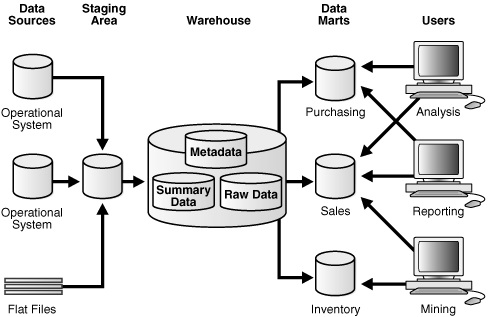
\includegraphics[width=88mm]{dwarehouse.jpg}
\end{figure}

This type of concept may seem convoluted to the average client, but what will make sense is how it will affect their organisations financially. Inmon states[16], that Data Warehousing significantly reduces the cost of information, with the result that organisations that use a Data Warehouse, can access a specific piece of information for \$100, as apposed to an organisation that doesn't have a Data Warehouse, who will access the same piece of information for \$10,000. 

\subsection{Benefits of Big Data \& Analytics}
If we analyse the information detailed in this review, it becomes clear that there are benefits to organisations who invest time and money in Big Data and Data Analysis. Here are some of the key benefits;

\begin{enumerate}
	\item \textbf{Cost Reduction:}\\ As outlined in the last section, Data Warehousing  and Data Analysis in general can yield substantial financial savings. But it's not just with implementation that's cost effective. According to Thomas Davenport[17], most companies and organisations are using Big Data and Warehousing to accompany their existing databases, as apposed to replacing the traditional architecture that's currently insitu. This is a huge cost reducing benefit from a maintenence perspective alone. \\
	
	\item \textbf{Improved Decision Making:}\\ To enable organisations to make proper decisions, they need information. The more information they have the better insight they have into what's been happening and be able to plan effectively for what could happen. To gain a visual insight into this and thanks to advancements in technology, snapshots can be taken of a specific period in time that display a visual perspective that can highlight peeks and troughs in particular areas of business. \\
	
	\item \textbf{New Products and Services}\\ With the explosion of Data in the last number of years, comes new products and services that can be tailored to customers needs. These services can help customers plan new advertising and marketing campaigns based on information they are receiving through Big Data Analysis. 
	 
\end{enumerate}


\subsection{Big Data, the next steps}
The creation of Data is unlikely to stop, so the next steps involve capturing as much relevant data in as many different ways as possible that will of course benefit companies and organisations. Apache Hadoop[18] is an open source framework for storing and processing large datasets using clusters. They use what's called a MapReduce method to condense or reduce large amounts of data into smaller parts. Although Hadoop have been around for a number of years, it's worth highlighting that they'll be involved in Big Data for the foreseable future due to the fact that they are highly involved in Big Data Warehousing, with many companies globally using their services[19]. \\

Apache Spark is worth mentioning as a contributor to the current and future world of Big Data. It's a fast, general purpose engine used for large-scale data processing[20]. It focuses on Speed that allows faster speeds than Hadoop MapRduce in memory; ease of use that enables applications to be written quickly in Java, Scala, Python and R; Generality, which allows you to combine libraries such as SQL and machine learning programs into one application[20]. Apache Spark is currently being used by companies such as Amazon, Yahoo, Nokia, NASA JPL(Jet Propulsion Lab) and Hitachi Solutions[21].


\section{Conclusion}
In this paper, we've had an in depth look into the world of Big Data and Data Analytics. Firstly we looked at how data is used by companies and organisations and gained some knowledge about how data works with the help of some interesting statistical analysis. We looked at Data in it's most basic form and looked at some size comparisons. We've discussed in great detail about Big Data, Data Analysis, Data Mining and how data operates on a much larger scale with the help of Data Warehousing. We outlined that reduction in cost and improved decision making were key benefits as a result of Big Data Analysis and finally we looked at some key new technologies that are working with large data sets and data warehousing to produce more efficient results. 

Upon reflection and based on the topics covered in this review, one might see that everything is a bi-product or result of another action with regard to Big Data. Essentially what this means is that as data creation accelerates, it creates a need in other areas. We create more data, we need to store it somewehere and as this data grows it needs to be searched for something useful and of course with this creates a need for employers to fill gaps by employing more people as required. Based on the rate at which technology is advancing, it's fair to estimate that data will continue to grow and as it grows, humans will find a way to evolve with it in order to benefit from it. 


\begin{thebibliography}{1}

\bibitem{IEEEhowto}
OECD (2013) New sources of growth- knowledge based capital. OECD, Paris. 
http://www.oecd.org/sti/inno/knowledge-based-capital-synthesis.pdf.

\bibitem{IEEEhowto}
Harness the Power of Big Data The IBM Big Data Platform
https://www-01.ibm.com/software/data/bigdata/what-is-big-data.html

\bibitem{IEEEhowto}
http://www.cam.ac.uk/research/discussion/talkin-bout-a-revolution-how-to-make-the-digital-world-work-for-us

\bibitem{ITEEEhowto}
Amatriain X (2013) Beyond Data: from user information to business value through personalized recommendations
and consumer science, CIKM’13. San Francisco, CA, USA

\bibitem{IEEEhowto}
Seizing the data opportunity: A strategy for UK data capability
bis-13-1250-strategy-for-uk-data-capability-v4.pdf

\bibitem{IEEEhowto}
http://www.asciitable.com

\bibitem{IEEEhowto}
How Much data.pdf
Release date: October 27, 2003. © 2003 Regents of the University of California

\bibitem{IEEEhowto}
Fayyad UM, Piatetsky-Shapiro G, Smyth P. From data mining to knowledge discovery in databases. AI Mag.1996

\bibitem{IEEEhowto}
TDWI Best Practices Report Next Generation Data Warehouse Platforms (Q4 2009), available on tdwi.org.

\bibitem{IEEEhowto}
Big Data Analytics by Philip Russom 2011
http://www.sas.com/content/dam/SAS/en\_us/doc/research2/big-data-analytics-105425.pdf

\bibitem{IEEEhowto}
https://docs.oracle.com/cd/B28359\_01/datamine.111/b28129/process.htm

\bibitem{IEEEhowto}
Tsai C-W, Lai C-F, Chiang M-C, Yang L. Data mining for internet of things: a survey. IEEE Commun Surveys Tutor.
2014;16

\bibitem{IEEEhowto}
SOME METHODS FOR CLASSIFICATION AND ANALYSIS OF MULTIVARIATE OBSERVATIONS by J Macqueen, University of California
https://pdfs.semanticscholar.org/a718/b85520bea702533ca9a5954c33576fd162b0.pdf

\bibitem{IEEEhowto}
Krishna K, Murty MN. Genetic k-means algorithm. IEEE Trans Syst Man Cyber Part B Cyber. 1999;

\bibitem{IEEEhowto}
https://docs.oracle.com/cd/B10500\_01/server.920/a96520/concept.htm

\bibitem{IEEEhowto}
Building the Data Warehouse Third Edition, W.H.Inmon, 2002

\bibitem{IEEEhowto}
Competing on Analytics by Thomas H. Davenport
http://www.milwaukeespin.com/Files/competing-on-analytics.pdf

\bibitem{IEEEhowto}
Hadoop. http://hadoop.apache.org/

\bibitem{IEEEhowto}
http://wiki.apache.org/hadoop/PoweredBy

\bibitem{IEEEhowto}
http://spark.apache.org/

\bibitem{IEEEhowto}
https://cwiki.apache.org/confluence/display/SPARK/Powered+By+Spark

\end{thebibliography}

\end{document}
